\part ¿Cu\'al es la distancia entre -3.9 y -4.7?

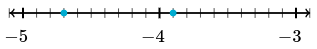
\includegraphics[width=0.8\linewidth]{Images/dist_nums_01}

\begin{minipage}[t]{0.9\linewidth}
    \begin{solutionbox}{6.5cm}
        % {\small
        Para encontrar la distancia entre 2 n\'umeros, s\'olo hay que restar el n\'umero mayor menos el n\'umero menor.
        En este ejercicio, el n\'umero mayor es el -3.9, ya que se encuentra a la derecha del -4.7, y por ello -4.7 es el menor. Entonces
        % }
        \begin{align*}
            d & = |-3.9-(-4.7)| \\
              & =  |-3.9 + 4.7| \\
              & = | 0.8 |       \\
              & = 0.8
        \end{align*}
    \end{solutionbox}
\end{minipage}